% %
% Adopted from:
%https://www.overleaf.com/latex/templates/refman-format-technical-reference-manuals/jjrfdfpyxzvz
%

\documentclass[twoside,a4paper]{refart}

\usepackage{graphicx,psfrag,verbatim,float} %In an effort to make figures work.

\usepackage{makeidx}
\usepackage{hyperref}
%The following to enable line wrapping compared to \verb|sometext|...
\usepackage{listings}
\usepackage{amsmath,amssymb,amsfonts}
\lstset{
basicstyle=\ttfamily,
columns=flexible,
breaklines=true
}


\title{Tool for validating a batch of data}
\author{University of Oulu, IMS \\
Markus Neuvonen \\
markus.neuvonen@oulu.fi \\
v1.0\\
\date{\today}}


\emergencystretch1em  %To get rid of box badness warnings?
\pagestyle{myfootings} %Visualization only...
\makeindex %To get rid of unnecessary warning


\begin{document}
\maketitle
\begin{abstract}
        This tool distributions is made as a part of COGNITWIN project WP4. This tool can be used for data validation of batch of numeric data. Invalid data entries can be identified and resolved, frozen measurement values can be detected and, most importantly, outlier candidates in the data set can be identified. The technical approach of this package is by a single Matlab class that handles the functionality as methods.
\end{abstract}



\section{Matlab class}
\index{validateBatch.m}\marginlabel{validateBatch.m:}
\verb|CLASS| Class definition file. Initializes an object when given a table containing a batch of data. Object properties can then be enquired and data validation methods applied.

\marginlabel{Syntax:}
\verb|myDataObject = validateBatch(givenDataTable);| creates an object containing provided batch of data.

\marginlabel{Input arguments:} Only one input argument is required, a Matlab table with desired data batch to validate. Note: numeric data variables with multiple columns are not supported in input table.

\marginlabel{Output arguments:} The data validation tool object containing the provided data and methods to manipulate it.

\subsection{Properties}
\index{metaBatch}\marginlabel{metaBatch:}
\verb|PROPERTY| table containing only the meta data part of original table (for example time stamps, comments etc.).
\marginlabel{Syntax:}
\verb|T = myDataObject.metaBatch;| outputs a Matlab table containing only the non-numeric variables.

\index{numericBatch}\marginlabel{numericBatch:}
\verb|PROPERTY| table containing only the numeric data part of original table.
\marginlabel{Syntax:}
\verb|T = myDataObject.numericBatch;| outputs a Matlab table containing only the numeric variables.

\subsection{Other required files}
This tool requires no other files to run. However, an installation of \emph{CVX}, a Matlab--based modeling system for convex optimization, is required.


\section{Methods}
\index{setFaultyEntriesParams}\marginlabel{setFaultyEntriesParams:}
\verb|METHOD| choose how to handle invalid data (NaN etc.).

\marginlabel{Syntax:}
\verb|myDataObject = myDataObject.setFaultyEntriesParams(option);| currently supports two options; 'remove' (default option) for removing the samples from data that contain invalid data, and 'zoh', which applies zero--order hold to overwrite the invalid data.

\marginlabel{Examples:}
\verb|myDataObject = myDataObject.setFaultyEntriesParams('zoh');| sets the next invalid data handling to act according to zero--order hold method.

\index{getFaultFreeData}\marginlabel{getFaultFreeData:}
\verb|METHOD| returns table of numeric data that has been processed according to faulty entry parameter.

\marginlabel{Syntax:}
\verb|T = myDataObject.getFaultFreeData();|

\marginlabel{Output arguments:}
\verb|T| table containing the numeric data of provided batch after invalid data hadling.

\index{setStuckValueParams}\marginlabel{setStuckValueParams:}
\verb|METHOD| configures stuck value detection with desired parameters.

\marginlabel{Syntax:}
\verb|myDataObject = myDataObject.setStuckValueParams(n,tol);|

\marginlabel{Input arguments:}
\verb|n| Integer amount of consecutive same values in a row accepted before determining a value to be stuck. Default value 10.

\verb|tol| Relative tolerance of how small changes are ignored. Default value $10^{-6}$.

\index{getStuckValues}\marginlabel{getStuckValues:}
\verb|METHOD| provides binary table indicating stuck values (1 = stuck, 0 = OK).

\marginlabel{Syntax:}
\verb|T = myDataObject.getStuckValues();|

\marginlabel{Output arguments:}
\verb|T| table containing binary indicator of the stuck status of numeric data.

\index{getOutlierCandidates}\marginlabel{getOutlierCandidates:}
\verb|METHOD| returns binary vector indicating outlier candidates (1 = candidate, 0 = not candidate) in the provided data.

\marginlabel{Syntax:}
\verb|[v,myDataObject] = myDataObject.getOutlierCandidates(n,tol,options);|

\marginlabel{Input arguments:}
\verb|n| Integer amount of consecutive ellipsoidal pealing procedures to be made. Note, relative to the initial, faulty data processed data set; so if called in iterative loop, value of $n$ must grow by one in each iteration. Method saves previously calculated results and does not need to re--do them as more layers are pealed (requires using the optional object output).

\verb|tol| Absolute tolerance of how close to the minimum volume ellipsoid a given point must be in order to be labeled an outlier candidate. Default value $10^{-5}$.

\verb|options| Optional name--value pairs. Currently supports only logical 'doPlot' pair (default value false). If value is set to true and data has two (or three) variables a 2D (3D) figure is produced showing the data and the found minimum volume ellipsoid covering them.

\marginlabel{Output arguments:}
\verb|v| a vector that is as long as amount of samples in original data. For sample is labelled either to be an outlier candidate (value 1) within the given amount of layers pealed or not (value 0).

\verb|myDataObject| optional output. Needs to be used in order to reuse the results from pealing earlier layers.

\marginlabel{Examples:}
\verb|v = myDataObject.getOutlierCandidates(1,'doPlot',true);| outputs the vector containing information which samples are outlier candidates with respect to first ellipsoidal pealing of the data. It also prints out a figure demonstrating the data. Note: here the data displayed is only that of the latest ellipsoidal pealing (i.e. not the full original data if pealing more layers than 1). Figure~\ref{fig:3d} is generated when ten samples of three variables are used as input data, and output \verb|v = [ 0 1 1 1 1 0 1 1 0 1]|$^T$.

\begin{figure}[H]
\begin{center}
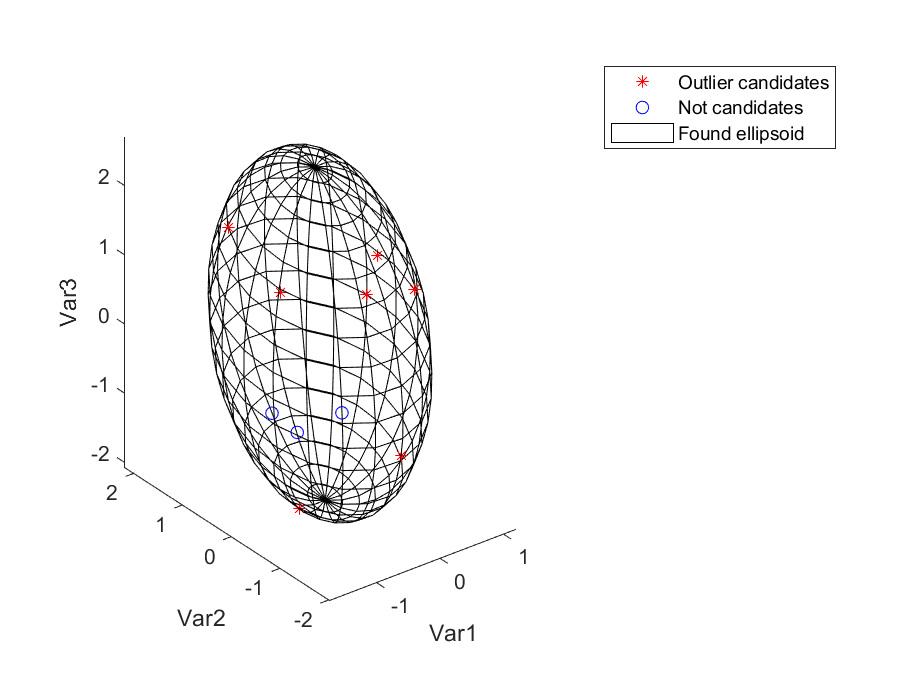
\includegraphics[width = 0.8\textwidth]{ep3d}
\end{center}
\caption{Visual overview of simple ellipsoidal pealing of three variables.}
\label{fig:3d}
\end{figure}

\printindex
\end{document} 